% !TeX program = lualatex
% !TeX encoding = utf8
% !TeX spellcheck = uk_UA
% !BIB program = bibler

\documentclass[onlytextwidth]{beamer}
\usetheme{Electromagnetism}
\usepackage{Electromagnetism}

%============================================================================
\title[Лекції електрики та магнетизму]{\huge\bfseries Електромагнітні хвилі}
\subtitle{Лекції з електрики та магнетизму}
\author{Пономаренко С. М.}
\date{}
%============================================================================
\graphicspath{{pictures/}}
\begin{document}
\begin{frame}[plain]
	\maketitle
\end{frame}

% ============================== Слайд ## ===================================
\begin{frame}{Хвильові рівняння}{Виведення}\small
	\begin{block}{}\justifying
		Розглянемо електромагнітне поле в однорідній ділянці простору, де немає вільних зарядів і струмів провідності.
	\end{block}
	\begin{columns}
		\begin{column}{0.45\linewidth}
			\begin{block}{}\justifying
				\begin{equation*}
					\begin{cases}
						\Div\Bfield = 0,                          \\
						\alert<1>{\Rot\Efield = -\frac1c\parttime{\Bfield}}, \\
						\Div\Dfield = 0,                          \\
						\alert<2>{\Rot\Hfield = \frac1c\parttime{\Dfield}}.
					\end{cases}
				\end{equation*}
				Врахуємо також матеріальні рівняння $\Dfield = \epsilon\Efield$, $\Bfield = \mu\Hfield$.
			\end{block}
		\end{column}
		\quad
		\begin{column}{0.55\linewidth}
			\begin{overprint}
				\onslide<1>
				\begin{block}{}
					До другого рівняння застосуємо операцію $\Rot$:
					\begin{equation*}
						\Rot\Rot\Efield = - \frac1c \parttime{} \Rot\Bfield.
					\end{equation*}
					\begin{equation*}
						\Rot\Rot\Efield =\Grad\Div\Efield - \nabla^2\Efield.
					\end{equation*}
					\begin{equation*}
						- \frac{\mu}c \parttime{}\Rot\Hfield = - \frac{\epsilon\mu}{c^2}\pparttime{\Efield}  .
					\end{equation*}
				\end{block}
				\onslide<2>
				\begin{block}{}
					До четвертого рівняння застосуємо операцію $\Rot$:
					\begin{equation*}
						\Rot\Rot\Hfield = + \frac1c \parttime{} \Rot\Dfield.
					\end{equation*}
					\begin{equation*}
						\Rot\Rot\Hfield =\Grad\Div\Hfield - \nabla^2\Hfield.
					\end{equation*}
					\begin{equation*}
						\frac{\mu}c \parttime{}\Rot\Dfield = - \frac{\epsilon\mu}{c^2}\pparttime{\Hfield}  .
					\end{equation*}
				\end{block}
			\end{overprint}
		\end{column}
	\end{columns}
	\begin{overprint}
		\onslide<1>
		\begin{block}{}
			Приходимо до рівняння для електричного поля:
			\begin{equation*}
				\nabla^2\Efield = \frac{1}{v^2}\pparttime{\Efield}, \quad \text{де}\ \frac{c}{\sqrt{\epsilon\mu}}.
			\end{equation*}
		\end{block}
		\onslide<2>
		\begin{block}{}
			Рівняння для магнітного поля:
			\begin{equation*}
				\nabla^2\Hfield = \frac{1}{v^2}\pparttime{\Hfield}, \quad \text{де}\ \frac{c}{\sqrt{\epsilon\mu}}.
			\end{equation*}
		\end{block}
	\end{overprint}
\end{frame}
% ===========================================================================

% ============================== Слайд ## ===================================
\begin{frame}{Хвильові рівняння}{}\small
	\begin{block}{}\justifying
		Рівняння вигляду:
		\begin{equation*}
			\begin{cases}
				\nabla^2\Efield = \frac{1}{v^2}\pparttime{\Efield}, \\
				\nabla^2\Hfield = \frac{1}{v^2}\pparttime{\Hfield}.
			\end{cases}
		\end{equation*}
		називаються хвильовими рівняннями. Вони описують процес поширення величин $\Efield$ та $\Hfield$ у просторі та часі зі швидкістю:
		\begin{equation*}
			v= \frac{c}{\sqrt{\epsilon\mu}}.
		\end{equation*}
		Такий процес називається \alert{електромагнітною хвилею}.
		У вакуумі $\epsilon=\mu=1$, а тому швидкість поширення хвилі буде $v = c =3\cdot10^{10}$~см/с. В середовищі для якого $\epsilon, \mu > 1$, а тому
		швидкість поширення буде меншою ніж у вакуумі $v < c$ на величну:
		\begin{equation*}
			n = \sqrt{\epsilon\mu},
		\end{equation*}
		яка називається \alert{абсолютним показником заломлення середовища}.
	\end{block}
\end{frame}
% ===========================================================================

% =================================================
\begin{frame}[t]{Плоскі електромагнітні хвилі}
	Розв'язком хвильових рівнянь, що описують плоскі хвилі є функції вигляду:
	\begin{onlyenv}<1-3>
		\begin{align}
			\vect{E} & = \vect{E}_m e^{i(\omega t - \vect{k}\vect{r})} \label{Ew} \\
			\vect{B} & = \vect{B}_m e^{i(\omega t - \vect{k}\vect{r})} \label{Bw}
		\end{align}
	\end{onlyenv}

	% -------------------------------------------------
	\begin{onlyenv}<1>

		\begin{center}
			\begin{tikzpicture}[scale=0.75, >=latex]
				\clip (-1,-1) rectangle (6,5);
				\draw[->] (0, -1) to (0,5) node[below left] {$y$};
				\draw[->] (-1, 0) to (6,0) node[below left] {$x$};
				\foreach \i in {0,1,...,5} {
						‎\draw[domain=-1:30, smooth, variable=\x, blue] plot ({\x}, {-\x + \i}) ;
					}
				\coordinate (K) at (1.5, {-1.5 + 4});
				\draw[->] (0,0) -- node[left=1pt] {$\vect{r}$} (K);
				\draw[->, red, double] (K) -- ++(45:1) node[right] {$\k$};
			\end{tikzpicture}
		\end{center}
	\end{onlyenv}

	% -------------------------------------------------
	\begin{onlyenv}<2>
		% Electromagnetic wave - colored
		\begin{tikzpicture}[>=latex, x=(-15:1.2), y=(90:1.0), z=(-150:1.0),
				line cap=round, line join=round,
				axis/.style={black, thick,->},
				vector/.style={>=stealth,->}, scale=0.8]
			\large
			\def\A{1.5}
			\def\nNodes{5} % use even number
			\def\nVectorsPerNode{8}
			\def\N{\nNodes*40}
			\def\xmax{\nNodes*pi/2*1.01}
			\pgfmathsetmacro\nVectors{(\nVectorsPerNode+1)*\nNodes}


			\def\drawENode{ % draw E node and vectors with some offset
				\draw[red,very thick,variable=\t,domain=\iOffset*pi/2:(\iOffset+1)*pi/2*1.01,samples=40]
				plot (\t,{\A*sin(\t*360/pi)},0);
				\foreach \k [evaluate={\t=\k*pi/2/(\nVectorsPerNode+1);
							\angle=\k*90/(\nVectorsPerNode+1);}]
				in {1,...,\nVectorsPerNode}{
						\draw[vector, help lines, red!80]  (\iOffset*pi/2+\t,0,0) -- ++(0,{\A*sin(2*\angle+\iOffset*180)},0);
					}
			}
			\def\drawBNode{ % draw B node and vectors with some offset
				\draw[blue,very thick,variable=\t,domain=\iOffset*pi/2:(\iOffset+1)*pi/2*1.01,samples=40]
				plot (\t,0,{\A*sin(\t*360/pi)});
				\foreach \k [evaluate={\t=\k*pi/2/(\nVectorsPerNode+1);
							\angle=\k*90/(\nVectorsPerNode+1);}]
				in {1,...,\nVectorsPerNode}{
						\draw[vector,help lines, blue!80]  (\iOffset*pi/2+\t,0,0) -- ++(0,0,{\A*sin(2*\angle+\iOffset*180)});
					}
			}

			% main axes
			\draw[axis] (0,0,0) -- ++(\xmax*1.1,0,0) node[right] {$x$};
			\draw[axis] (0,-\A*1.4,0) -- (0,\A*1.4,0) node[right] {$y$};
			\draw[axis] (0,0,-\A*1.4) -- (0,0,\A*1.4) node[above left] {$z$};

			% small axes
			\def\xOffset{{(\nNodes-2)*pi/2}}
			\def\yOffset{\A*1.2}
			\def\zOffset{\A*1.2}
			\draw[axis,black] (\xOffset,\yOffset,-\zOffset) -- ++(\A*0.6,0,0) node[right,align=center] {$\k$}; %\\propagation
			\draw[axis,red]  (\xOffset,\yOffset,-\zOffset) -- ++(0,\A*0.6,0) node[right] {$\Efield$};
			\draw[axis,blue]   (\xOffset,\yOffset,-\zOffset) -- ++(0,0,\A*0.6) node[above left] {$\Bfield$};

			% equation


			% draw (anti-)nodes
			\foreach \iNode [evaluate={\iOffset=\iNode-1;}] in {1,...,\nNodes}{
					\ifodd\iNode \drawBNode \drawENode % E overlaps B
					\else        \drawENode \drawBNode % B overlaps E
					\fi
				}

		\end{tikzpicture}
	\end{onlyenv}

	% -------------------------------------------------
	\begin{onlyenv}<3>

		Підставимо \eqref{Ew} та \eqref{Bw} в рівняння Максвелла. Диференціальні операції заміняються на:

		\begin{equation*}
			\vect{\nabla} \to -i\vect{k}, \quad \frac{\partial}{\partial t} \to i\omega
		\end{equation*}

		\begin{equation*}
			\vect{k}\times\Efield    =\frac\omega{c}  \Bfield,    \quad
			-\vect{k}\times \Hfield =  \frac\omega{c} \epsilon\Efield
			%    k^2 \Efield &= \frac{n^2}{c^2} \omega^2 \Efield, \quad k^2 = \frac{\omega^2}{v^2}
		\end{equation*}


		\begin{equation*}
			k =  \frac{\sqrt{\epsilon\mu}}{c} \omega = \frac{n}{c} \omega = \frac{\omega}{v}, \quad n E_m = B_m, \quad \sqrt{\epsilon} E_m = \sqrt{\mu} H_m
		\end{equation*}
	\end{onlyenv}

	% -------------------------------------------------
	\framesubtitle<4>{Енергія хвилі та вектор Пойнтінга}
	\begin{onlyenv}<4>
		\begin{equation*}
			\vect{k}\times\Efield    =\frac\omega{c}  \Bfield,    \quad
			-\vect{k}\times \Hfield =  \frac\omega{c} \epsilon\Efield
			%    k^2 \Efield &= \frac{n^2}{c^2} \omega^2 \Efield, \quad k^2 = \frac{\omega^2}{v^2}
		\end{equation*}


		\begin{equation*}
			k =  \frac{\sqrt{\epsilon\mu}}{c} \omega = \frac{n}{c} \omega = \frac{\omega}{v}, \quad n E_m = B_m, \quad \sqrt{\epsilon} E_m = \sqrt{\mu} H_m
		\end{equation*}
		Густина енергії (амплітуда)
		\begin{equation*}
			w_m = \frac{\epsilon E_m^2}{8\pi} + \frac{\mu H_m^2}{8\pi}, \quad  \sqrt{\frac{\epsilon}{\mu}} E_m = H_m, \quad w_m = \frac{\epsilon E_m^2}{4\pi} = \frac{\mu H_m^2}{4\pi}.
		\end{equation*}

		Вектор вектор Пойнтінга $ \vect{\Pi} = \frac{c}{4\pi}[\Efield\times\Hfield] $:

		%        \begin{equation*}
		%            \Efield = - \frac{c}{\epsilon \omega} \vect{k}\times\Hfield
		%        \end{equation*}

		\begin{equation*}
			\vect{\Pi} =  \frac{c^2}{4\pi\epsilon \omega} \Hfield\times\vect{k}\times\Hfield = \frac{c^2}{4\pi\epsilon \omega} H^2 \vect{k} =
			\frac{c}{\omega} \frac{1}{\epsilon\mu}\left( \frac{\mu H^2}{4\pi}\right)   c \vect{k} = w \frac{c}{\sqrt{\epsilon\mu}} \frac{\vect{k}}{k}= w
			\vec{v}.
		\end{equation*}
	\end{onlyenv}
\end{frame}
% ============================== Слайд ## ===================================






% ============================== Слайд ## ===================================
\begin{frame}{Тиск світла}{}\small
	\begin{block}{}\justifying
		Максвел теоретично показав, що електромагнітні хвилі, відбиваючись чи поглинаючись тілами, на які  вони падають, чинять на них тиск. Цей тиск виникає внаслідок впливу магнітного поля хвилі на електричні струми, що збуджуються електричним полем тієї самої хвилі.
	\end{block}
	\vspace*{-1.25em}
	\begin{columns}
		\begin{column}{0.4\linewidth}
			\begin{center}
				\includegraphics[width=1\linewidth]{pictures/elmagpresure}
			\end{center}
		\end{column}
		\begin{column}{0.6\linewidth}
			\begin{block}{}\justifying\small
				Електричне поле хвилі збуджує електричний струм густиною $ \vect{j} = \sigma\Efield $ ($ \vect{F} = e\Efield $). Внаслідок цього на
				об'єму середовища діє сила Ампера $ d\vect{F} = \frac1c[\vect{j}\times\Bfield] dV$, спрямована убік поширення хвилі. Ця сила та викликає
				тиск електромагнітної хвилі.
        	\end{block}
		\end{column}
	\end{columns}
            \begin{block}{}\justifying\small
				\begin{overprint}
					\onslide<1>
					У випадку поглинання вся енергія, яка падає за секунду на поверхню $wv dS$ тіла, перетворюється на теплову $ jE dV $:
					\begin{equation*}
						dF = \frac1c j \frac{c}{v}E = \frac1vjE = \frac1v wvdS = w dS,
					\end{equation*}
					звідки тиск $ p = \frac{dF}{dS} = w $
					\onslide<2>
					У випадку часткового відбивання, тиск дорівнює
					\begin{equation*}
						p = w (1 + \rho),
					\end{equation*}
					де $ \rho = 0 \ldots 1$ --- коефіцієнт відбивання.
				\end{overprint}
			\end{block}
\end{frame}

\begin{frame}{Тиск світла}{Дослід Лебедєва}\small
\begin{block}{}\justifying
    Петро Миколайович Лебедєв в 1899 р. вперше виміряв світловий тиск.
\end{block}
	\begin{columns}
		\begin{column}{0.6\linewidth}
            \begin{block}{}\justifying
			Він підвісив на тонкій нитці коромисло з парою крилець на кінцях:
			поверхня в одного з них була зачорненою, забезпечуючи майже повне поглинання, а в іншого --- дзеркальною, забезпечуючи повне відбивання.
			Підвіс з крильцями утворив чутливі крутильні терези, що поміщаються в посудину, повітря в якому було відкачано.
            \end{block}
		\end{column}
		\begin{column}{0.4\linewidth}\centering
			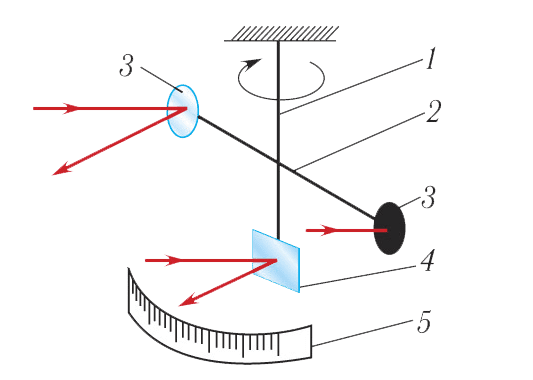
\includegraphics[width=\linewidth]{LebedevExp}
		\end{column}
	\end{columns}

	\begin{block}{}\justifying
		Світло практично повністю відбивалося від дзеркальної поверхні та його тиск на дзеркальне крильце було вдвічі більше, ніж на зачорнене. Внаслідок цього створювався момент сил, що повертає коромисло. Вимірюючи кут повороту коромисла, можна було виміряти силу, що діяла на крильця, а отже, визначити світловий тиск.
	\end{block}
	{\tiny \url{https://youtu.be/Dr07pTIoue8}}
\end{frame}

% ===========================================================================
\begin{frame}{Тиск світла}{Сонячні вітрила}\small
	\begin{onlyenv}<1>
		\begin{block}{}\justifying
			Сонячне вітрило --- пристрій, що використовує тиск сонячного світла чи лазера на дзеркальну поверхню для приведення в рух космічного апарату.

			\bigskip

			Тиск сонячного світла надзвичайно малий (на Земній орбіті --- близько $5\cdot10^{-6}$~Па) і зменшується пропорційно квадрату відстані від Сонця. В ролі вітрила використовувались сонячні батареї або радіатори системи терморегуляції.
		\end{block}

		\begin{center}
			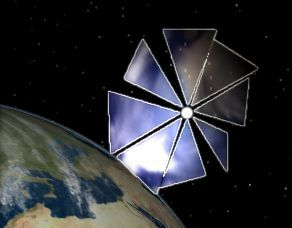
\includegraphics[width=0.4\linewidth]{Cosmos_solar_sail}
		\end{center}

		{\tiny \url{https://youtu.be/U0_wjnmlmRg}}
	\end{onlyenv}
	\begin{onlyenv}<2>
		\begin{block}{}\justifying
			Вчені з Австралійського національного університету запропонували спосіб запуску для космічного вітрильника до найближчої зірки Альфи Центавра в рамках проекту Breakthrough Starshot. За їх задумом, надати необхідну швидкість апарату допоможе фотонний двигун --- система, що сумарно включає до 100 мільйонів лазерів.
		\end{block}
		\begin{center}
			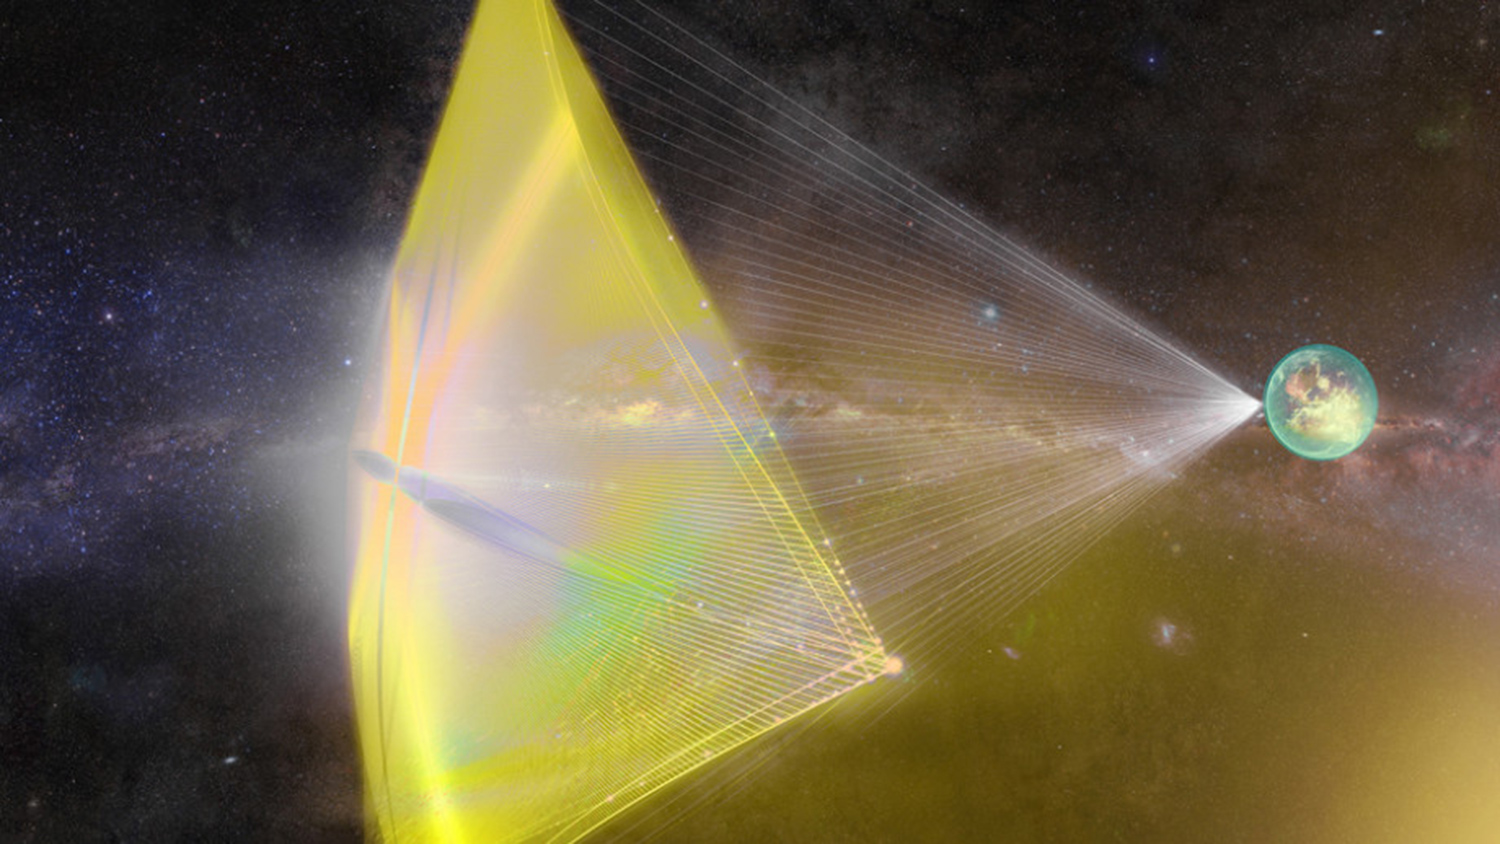
\includegraphics[width=0.5\linewidth]{Starshot-light-sail_Breakthroughinitiatives}
		\end{center}
		\begin{block}{}\justifying
			Подорож до Альфи Центавра за допомогою звичайних способів переміщення триватиме близько 100 років. Дістатись до Альфи Центавра за допомогою космічного вітрильника на фотонному двигуні передбачається за 20 років зі швидкістю в $ 0.2 c $.
		\end{block}
		{\tiny      \href{https://opg.optica.org/josab/fulltext.cfm?uri=josab-38-5-1477&id=450064}{Journal of the Optical Society of America B}.}
	\end{onlyenv}
	\begin{onlyenv}<3>
		\begin{block}{}\justifying
			Тиск світла відіграє велику роль в астрономічних та атомних явищах. В астрофізиці тиск світла поряд із тиском газу забезпечує стабільність зірок, протидіючи силам гравітації. Дія тиску світла пояснюються деякі форми кометних хвостів. До атомних ефектів відноситься так звана світлова віддача, яку відчуває збуджений атом під час випромінювання фотона.
		\end{block}
		\begin{columns}\centering
			\begin{column}{0.5\linewidth}\centering
				\includegraphics[width=0.75\linewidth]{Star}
			\end{column}
			\begin{column}{0.5\linewidth}\centering
				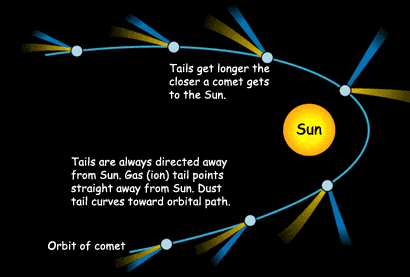
\includegraphics[width=0.75\linewidth]{Comet}

				\begin{block}{}\tiny\centering
					Товстий білий хвіст комети Гейла-Боппа складається з частинок пилу, і утворюється завдяки тиску світла. Другий, тонкий і блакитний складається з іонів і створюється сонячним вітром.
				\end{block}
			\end{column}
		\end{columns}
	\end{onlyenv}
\end{frame}
% ===========================================================================





% ============================== Слайд ## ===================================
\begin{frame}{Імпульс електромагнітного поля}{}
	\begin{block}{}\justifying\small
		Поле має енергію; так само в одиниці об'єму воно має якийсь імпульс. Оскільки електромагнітна хвиля чинить тиск на речовину, остання набуває певного імпульсу. Але в замкнутій системі, що складається з речовини та електромагнітної хвилі, виникло б порушення закону збереження імпульсу, якби імпульс мала лише речовина.
	\end{block}

	Для електромагнітної хвилі у вакуумі вектор Пойнтінга.
	\begin{equation*}
		\Pi = w c \Rightarrow \frac{\Pi}{c^2} = \frac{w}{c}.
	\end{equation*}

	З релятивістської механіки $ E^2 = m^2c^4 + p^2c^2 $. Для частинки з нульовою масою (наприклад, фотона) $ m = 0 $, зв'язок енергії та імпульсу:
	\begin{equation*}
		E = p c \Rightarrow  p = \frac{E}{c}.
	\end{equation*}

	Порівнюючи дві останні формули, отримаємо вираз для густини імпульсу:
	\begin{equation*}
		\vect{g} = \frac{\vect{\Pi}}{c^2}, \quad [g] = \frac{\text{дин}\cdot\text{с}}{\text{см}^3}\, \text{(СГС)}
	\end{equation*}
\end{frame}
% ===========================================================================




% ============================== Слайд ## ===================================
\begin{frame}{Момент імпульсу поля}{}\scriptsize
	\begin{exampleblock}{\scriptsize Задача}\justifying
		Заряджений циліндричний конденсатор вміщений в зовнішнє однорідне магнітне поле з індукцією $ \Bfield $, що напрямлене вздовж його осі.
		Конденсатор має змогу вільно обертатись навколо своєї осі. Заряд конденсатора $ q $, радіус зовнішньої обкладки $ R $, радіусом внутрішньої
		можна знехтувати.  Маса конденсатора $ m $. Знайдіть вектор моменту імпульсу електромагнітного поля конденсатора. Знайдіть кутову швидкість, з
		якою буде обертатись конденсатор, при вимикання магнітного поля.
	\end{exampleblock}
	\begin{columns}
		\begin{column}{0.25\linewidth}
			\begin{center}
				\begin{tikzpicture}[scale=1.2, >=latex]
					\draw [fill=gray, fill opacity=.25]
					(180:1mm) coordinate (a)
					-- ++(0,-15mm) coordinate (b)
					arc (180:360:1mm and 0.25mm) coordinate (d)
					-- (a -| d) coordinate (c) arc (0:180:1mm and 0.25mm);
					\draw [fill=gray, fill opacity=.25]
					(0,0) coordinate (t) circle (1mm and 0.25mm);
					\draw [densely dashed] (d) arc (0:180:1mm and 0.25mm);

					\draw [thick]
					(180:7.5mm) coordinate (A)
					-- ++(0,-15mm) coordinate (B) %node [midway, right, inner sep=1pt] {$v$}
					arc (180:360:7.5mm and 2.625mm) coordinate (D)
					-- (A -| D) coordinate (C) arc (0:180:7.5mm and 2.625mm);
					\draw [thick]
					(0,0) coordinate (T) circle (7.5mm and 2.625mm);
					\draw [densely dashed] (D) arc (0:180:7.5mm and 2.625mm);

					\foreach[count=\j] \i in {-0.5, 0, 0.5} {
							\draw[blue, <-] (\i,5mm) \ifnum\j=2 node[above] {$\Bfield$} \fi -- ++(0,-25mm);
						}

					\foreach[count=\j] \i in {0, -0.5, -1, -1.5} {
							\draw[red, ->] (1mm,\i) -- ++(6.5mm,0) \ifnum\j=2 node[right] {$ \Efield $}\fi;
							\draw[red, ->] (-1mm,\i) -- ++(-6.5mm,0);
						}

					\draw (0,0) ellipse (1mm and 0.25mm);

					\draw[green!50!black, <-] (0,-0.75) [partial ellipse=110:430:4mm and 1.3mm] node[above, pos=0.2] {$ \vect{\Pi} $};

				\end{tikzpicture}
			\end{center}
		\end{column}
		\begin{column}{0.75\linewidth}
			\begin{block}{}\justifying
				Густина моменту імпульсу поля:
				\begin{equation*}
					\vec{\mathcal{L}} = \vect{r}\times\frac{\vect{\Pi}}{c^2} = \frac{1}{4\pi c} \vect{r}\times \Efield \times \Bfield = - \frac{1}{4\pi c}
					\Bfield (\vect{r}\cdot \Efield)
				\end{equation*}

				Електричне поле :
				\(\displaystyle
				E = \frac{2\lambda}{r} = \frac{2q}{rh}, \quad h - \text{висота циліндра}
				\)

				Модуль вектора імпульсу $ \vect{L} $:
				\begin{equation*}
					L = \iiint\limits_V\mathcal{L} dV = \frac{1}{4\pi c} B \frac{2q}{h} \pi R^2 h = \frac{qBR^2}{2c}, \quad \vect{L} = - \frac{qR^2}{2c}
					\Bfield
				\end{equation*}
			\end{block}
		\end{column}
	\end{columns}
	\begin{block}{}\justifying
		При вимиканні магнітного поля момент імпульсу має зберегтися, тому він перейде в обертання самого циліндра $ \vect{L} = mR^2\vec\omega
		$, а тому кутова швидкість:
		\(
		\displaystyle	\vec{\omega} = -\frac{q}{2mc}\vect{B}.
		\)
	\end{block}
\end{frame}
% ===========================================================================

\end{document}
